\chapter{Расчет потокораспределения и напряжений в узлах сети в нормальном режиме наименьших нагрузок}
\label{cha:40-low_loads}

\section{Расчет нагрузок на шинах низшего и среднего напряжений подстанции}

Возьмем значения активной мощности на шинах низшего и среднего напряжений, $tg\varphi_\textup{н}$ и $cos\varphi_\textup{с}$ из табл. \ref*{tab:tabl2}.

Активная нагрузка на шинах низшего напряжения (НН): $P_\textup{н} = 22,9 \cdot \alpha = 22,9\cdot 0,4 = 9,16 \; \text{МВт}$

Реактивная нагрузка на шинах НН вычисляется по формуле:
\begin{eqndesc}
	\begin{equation*}
		Q_\textup{н} = P_\textup{н}\cdot tg\varphi_\textup{н}\cdot \alpha = 22,9\cdot 0,44\cdot 0,4 = 4,03\; \text{МВар},
	\end{equation*}
	
	где $P_\textup{н}$ "--- активная нагрузка на шинах НН, \\
	$tg_{\varphi_{\text{н}}}$ "--- коэффициент реактивной мощности.
\end{eqndesc}

Активная нагрузка на шинах среднего напряжения (СН): $P_\textup{с} = 33\cdot 0,4 = 13,2\; \text{МВт}$

Реактивная нагрузка на шинах НН вычисляется по формуле:
\begin{eqndesc}
	\begin{equation*}
		Q_\textup{с} = \sqrt{S_c^2 - P_c^2} = \sqrt{\left(\frac{P_c}{cos\varphi_c}\right)^2 - P_c^2} = \sqrt{\left(\frac{13,2}{0,82}\right)^2 - 13,2^2} = 9,21\; \text{Мвар},
	\end{equation*}
	
	где $P_\textup{с}$ "--- активная мощность нагрузки на шинах СН, \\
	$cos_{\varphi_{\text{с}}}$ "--- коэффициент мощности нагрузки, \\
	$S_\textup{с}$ "--- полная мощность на шинах СН.
\end{eqndesc}

\section{Расчет режима наименьших нагрузок}

По условию, напряжение на источнике питания в режиме наименьших нагрузок составляет 97\%. Найдем напряжение ИП-ПС:
\[U_\textup{ИП-ПС} = U_\textup{ном} \cdot U_\textup{ИП}, \% = 110\cdot 0,97 = 106,7\; \text{кВ}\]

\textbf{1 этап}

В качестве начального приближения зададимся значениями напряжений на шинах СН и ВН, приведенными к стороне ВН, а так же напряжения в средней точке схемы замещения ТР, равными номинальному напряжению:
\[U_\textup{в}^{(0)} = U_\textup{н}^{{'}(0)} = U_\textup{с}^{{'}(0)} = U_0^{(0)} = U_\textup{ном} = 110\; \text{кВ}\]

\textbf{Луч среднего напряжения}

Мощность в конце луча СН:
\[S_c^{''} = P_c + jQ_c = 13,2 + j9,21 \; \text{МВА} \]

%Потеря мощности в сопротивлении рассчитывается по формуле:
%\begin{eqndesc}
%	\begin{equation}
%		\Delta S_{12} = \left(\frac{S_{12}^{(')('')}}{U_{(1)(2)}}\right)^2 \cdot Z_{12}
%		\label{eq:dS12}
%	\end{equation}
%	
%	где $S_12^{'}$ \--- мощность в начале участка 1-2, МВА, \\
%	$S_12^{''}$ \--- мощность в конце участка 1-2, МВА, \\
%	$U_1$ \--- напряжение в начале участка 1-2, кВ, \\
%	$U_2$ \--- напряжение в конце участка 1-2, кВ, \\
%	$Z_{12}$ \--- сопротивление участка 1-2, Ом.
%\end{eqndesc}

Определим потери мощности в сопротивлении луча СН по формуле \eqref{eq:dS12}:
\[\Delta S_c = \frac{(S_c^{''})^2}{U_\textup{ном}^2}\cdot Z_c = \frac{13,2^2+9,21^2}{110^2}\cdot 0,413 = 0,00884\; \text{МВт}\]

Определим мощность в начале луча СН:
\[S_c^{'} = S_c^{''} + \Delta S_c = 13,2 + j9,21 + 0,00884 = 13,2 + j9,21\; \text{МВА}\]

\textbf{Луч низшего напряжения}

Мощность в конце луча НН:
\[S_\textup{н}^{''} = P_\textup{н} + jQ_\textup{н} = 9,16 + j4,03 \; \text{МВА}\]

Потери мощности в сопротивлении луча НН:
\[\Delta S_\textup{н} = \frac{(S_\textup{н}^{''})^2}{U_\textup{ном}^2}\cdot Z_\textup{н} = \frac{9,16^2+4,03^2}{110^2}\cdot (0,413 + j10,3) = 0,00342 + j0,0853\; \text{МВА}\]

Определим мощность в начале луча НН:
\[S_\textup{н}^{'} = S_\textup{н}^{''} + \Delta S_\textup{н} = 9,16 + j4,03 + 0,00342 + j0,0853 = 9,16 + j4,12\; \text{МВА}\]

\newpage
\textbf{Луч высшего напряжения}

Мощность в конце луча ВН:
\[S_\textup{в}^{''} = S_c^{'} + S_\textup{в}^{'} = 13,2 + j9,21 + 9,16 + j4,12 = 22,4 + j13,3\; \text{МВА}\]

Потери мощности в сопротивлении луча ВН:
\[\Delta S_\textup{в} = \frac{(S_\textup{в}^{''})^2}{(U_\textup{ном})^2} \cdot Z_\textup{в} = \frac{22,4^2 + 13,3^2}{110^2} \cdot (0,413 + j17,9) = 0,0232 + j1,00\; \text{МВА} \]

Мощность в начале луча ВН:
\[S_\textup{в}^{'} = S_\textup{в}^{''} + \Delta S_\textup{в} = 22,4 + j13,3 + 0,0232 + j1,00 = 22,4 + j14,3\; \text{МВА}\]

Приведенная нагрузка подстанции:
\[S_\textup{прив} = S_\textup{в}^{'} + \Delta S_\textup{х} = 22,4 + j14,3 + 0,086 + j0,48 = 22,5 + j14,8\; \text{МВА}\]

Зарядная мощность в конце линии ИП-ПС:
\[\frac{Q_\textup{с.ИП-ПС}^{''}}{2} = \frac{U_\textup{ном}^2\cdot B_\textup{л}}{2} = \frac{110^2 \cdot 460,3\cdot 10^{-6}}{2} = 2,78\; \text{МВар} \]

Расчетная нагрузка подстанции:
\[S_p = S_\textup{прив} - j\frac{Q_\textup{с.ИП-ПС}^{''}}{2} = 22,5 + j14,8 - j2,78 = 22,5 + j12,0\; \text{МВА}\]

Мощность в конце линии ИП-ПС:
\[S_\textup{ИП-ПС}^{''} = S_p = 22,5 + j12,0\; \text{МВА}\]

Потери мощности в сопротивлении линии ИП:
\[\Delta S_\textup{ИП-ПС} = \frac{\left(S_\textup{ИП-ПС}^{''}\right)^2}{U_\textup{ном}^2}\cdot Z_\textup{л} = \frac{22,5^2 + 12,0^2}{110^2} \cdot (8,57 + j17,5) = 0,461 + j0,940\; \text{МВА}\]

Мощность в начале линии ИП-ПС:
\[S_\textup{ИП-ПС}^{'} = S_\textup{ИП-ПС}^{''} + \Delta S_\textup{ИП-ПС} = 22,5 + j12,0 + 0,461 + j0,940 = 23,0 + j12,9\; \text{МВА}\]

Зарядная мощность в начале линии ИП-ПС:
\[\frac{Q_\textup{с.ИП-ПС}^{'}}{2} = \frac{U_\textup{ИП-ПС}^2\cdot B_\textup{л}}{2} = \frac{106,7^2 \cdot 460,3\cdot 10^{-6}}{2} = 2,62\; \text{МВар}\]

Мощность, выдаваемая источником в сеть:
\[S_\textup{ИП-ПС} = S_\textup{ИП-ПС}^{'} - j\frac{Q_\textup{с.ИП-ПС}^{'}}{2} = 23,0 + j12,9 - j2,62 = 23,0 + j10,3\; \text{МВА}\]

\textbf{2 этап}

%Продольная составляющая вектора падения напряжения находится по формуле:
%
%\begin{equation}
%	\Delta U_{12} = \frac{P_{12}^{(')('')}\cdot R_{12} + Q_{12}^{(')('')}\cdot X_{12}}{U_{(1)(2)}}
%\end{equation}
%
Поперечной составляющей можем пренебречь, так как линия класса напряжения 110 кВ.

Продольная составляющая вектора падения напряжения на сопротивлении линии ИП-ПС:
\[\Delta U_\textup{ИП-ПС} = \frac{P_\textup{ИП-ПС}^{'}\cdot R_\textup{л} + Q_\textup{ИП-ПС}^{'}\cdot X_\textup{л}}{U_\textup{ИП-ПС}} = \frac{23,0\cdot 8,57 + 12,9\cdot 17,5}{106,7} = 3,96\; \text{кВ}\]

Напряжение на шинах ВН:
\[U_\textup{в} = U_\textup{ИП-ПС} - \Delta U_\textup{ИП-ПС} = 106,7 - 3,96 =  102,7\; \text{кВ}\]

Продольная составляющая вектора падения напряжения на сопротивлении луча высшего напряжения:
\[\Delta U_\textup{в} = \frac{P_\textup{в}^{'}\cdot R_\textup{т.в} + Q_\textup{в}^{'}\cdot X_\textup{т.в}}{U_\textup{в}} = \frac{22,4\cdot 0,413 + 14,3\cdot 17,9}{102,7} = 2,58\; \text{кВ}\]

Напряжение в средней точке схемы замещения трансформаторов:
\[U_\textup{0} = U_\textup{в} - \Delta U_\textup{в} = 102,7 - 2,58 = 100,1\; \text{кВ}\]

Продольная составляющая вектора падения напряжения на сопротивлении луча среднего напряжения:
\[\Delta U_\textup{с} = \frac{P_\textup{с}^{'}\cdot R_\textup{т.с} + Q_\textup{с}^{'}\cdot X_\textup{т.с}}{U_\textup{0}} = \frac{13,2\cdot 0,413 + 9,21\cdot 0}{100,1} = 0,0545\; \text{кВ}\]

Напряжение на шинах СН, приведенное к стороне ВН:
\[U_\textup{с}^{'} = U_\textup{0} - \Delta U_\textup{н} = 100,1 - 0,0545 = 100,0 \; \text{кВ}\]

Продольная составляющая вектора падения напряжения на сопротивлении луча низшего напряжения:
\[\Delta U_\textup{н} = \frac{P_\textup{н}^{'}\cdot R_\textup{т.н} + Q_\textup{н}^{'}\cdot X_\textup{т.н}}{U_\textup{0}} = \frac{9,16\cdot 0,413 + 4,12\cdot 10,3}{100,1} = 0,462\; \text{кВ}\]

Напряжение на шинах НН, приведенное к стороне ВН:
\[U_\textup{н}^{'} = U_\textup{0} - \Delta U_\textup{н} = 100,1 - 0,462 = 99,6 \; \text{кВ}\]

Полная расчетная схема замещения сети в нормальном режиме наименьшей нагрузки приведена на рис. \ref{fig:rezhim_NM}. 

\begin{sidewaysfigure}
	\centering
	\includegraphics[width=0.9\textwidth]{inc/svg/rezhim_NM}
	\caption{Полная схема замещения сети в режиме наименьших нагрузок}
	\label{fig:rezhim_NM}
\end{sidewaysfigure}